%-------------------------------------------------------------------------------
%-------------------------------------------------------------------------------
\begin{frame}\begin{center}
	\LARGE\textbf{True rate of return}
\end{center}\end{frame}
%-------------------------------------------------------------------------------
%-------------------------------------------------------------------------------
\begin{frame}
Suppose their is uncertainty about net earnings conditional on $s$ and actual lifetime earnings for someone with $s$ years of schooling are:

\begin{align*}
Y_s = \underbrace{\left[\sum^T_{x = 0}(1 + r)^{-x} Y(s, x)\right]}_{\bar{Y}_s}\epsilon_s
\end{align*}
\end{frame}
%-------------------------------------------------------------------------------
%-------------------------------------------------------------------------------
\begin{frame}
\begin{figure}[htp]\centering
\caption{Model structure}
\scalebox{0.35}{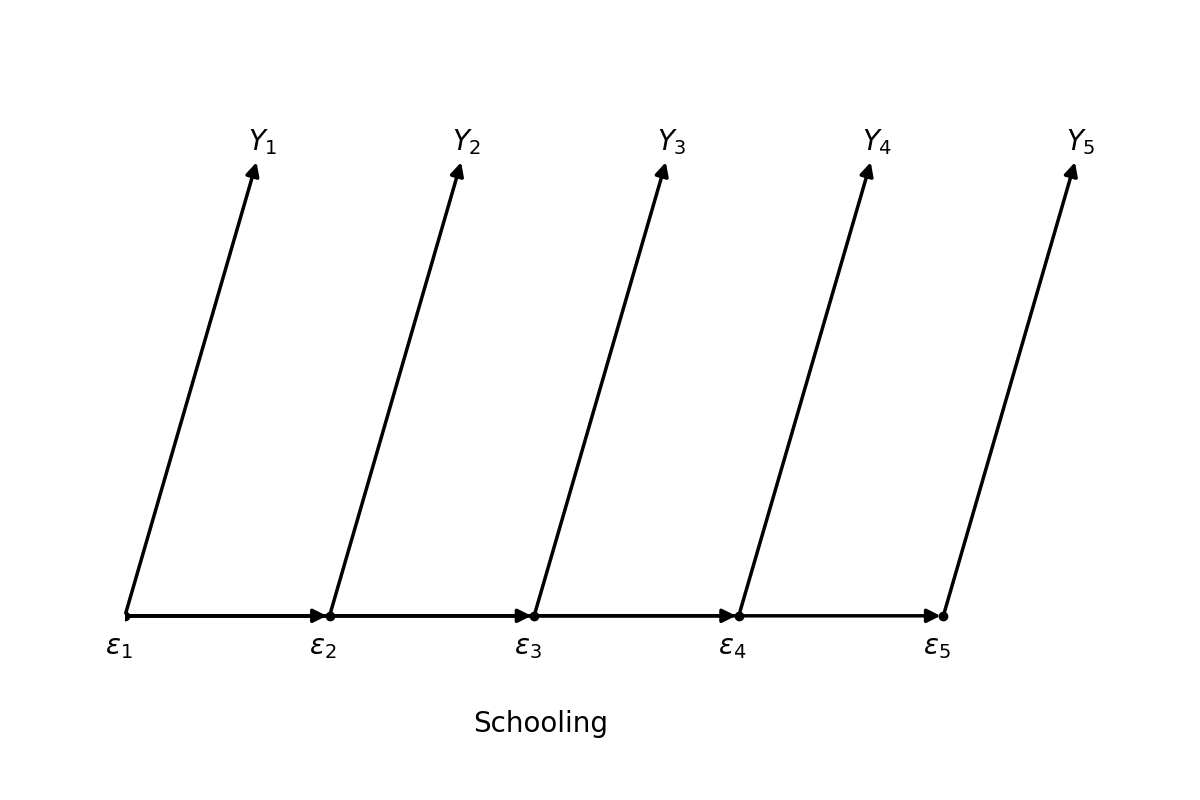
\includegraphics{fig-model-true-structure}}
\end{figure}
\end{frame}
%-------------------------------------------------------------------------------
%-------------------------------------------------------------------------------
\begin{frame}
The decision problem for a person with $s$ years of schooling given the sequential revelation of information is to complete another year of schooling if

\begin{align*}
Y_s \leq \frac{E_s(V_{s+1})}{1 + r}.
\end{align*}

\end{frame}
%-------------------------------------------------------------------------------
%-------------------------------------------------------------------------------
\begin{frame}
So the value of schooling level $s$, $V_s$, is

\begin{align*}
V_s = \max\left\{Y_s, \frac{E_s(V_{s+1})}{1 + r}\right\}
\end{align*}
for $s \leq \bar{S}$. At the maximum schooling level, $\bar{S}$, after all information is revealed, we obtain $V_{\bar{s}} = Y_{\bar{s}} = \bar{Y}_{\bar{s}}\epsilon_{\bar{s}}$.

\end{frame}
%-------------------------------------------------------------------------------
%-------------------------------------------------------------------------------
\begin{frame}
The endogenously determined probability of going on from school level $s$ to $s + 1$ is

\begin{align*}
p_{s + 1, s} = \Pr\left(\epsilon_s \leq \frac{E_s(V_{s + 1})}{(1 + r) \bar{Y}_s}\right),
\end{align*}
where $E_s(V_{s + 1})$ may depend on $\epsilon_s$ because it enters the agent's information set.
\end{frame}
%-------------------------------------------------------------------------------
%-------------------------------------------------------------------------------
\begin{frame}
Thus, the expected value of schooling level $s$ as perceived at current schooling $s-1$ is:

\begin{align*}
E_{s - 1}(V_s) & = \underbrace{(1 - p_{s + 1, s}) \bar{Y}_s E_{s - 1}\left(\epsilon\mid \epsilon \ge \frac{E_s(V_{s + 1})}{(1 + r)\bar{Y}_s}\right)}_{\text{direct return}} \\
 & + \underbrace{p_{s + 1, s} \left(\frac{E_{s - 1}(V_{s + 1})}{1 + r}\right)}_{\text{option value}}.
\end{align*}
\end{frame}
%-------------------------------------------------------------------------------
%-------------------------------------------------------------------------------
\begin{frame}\textbf{Objects of interest}\vspace{0.3cm}

\begin{itemize}
\item Option value
\begin{align*}
O_{s, s - 1} = \E_{s - 1}\left[V_s - Y_s\right]\\
\end{align*}
\item True rate of return
\begin{align*}
R_{s, s - 1} = \frac{\E_{s - 1}\left[V_s\right] - Y_{s - 1}}{Y_{s -1}}
\end{align*}
\end{itemize}
\end{frame}
%-------------------------------------------------------------------------------
%-------------------------------------------------------------------------------
\begin{frame}\textbf{Model specification}
\begin{align*}\begin{array}{l@{\qquad}l}
\ln(\epsilon_s) \sim \N(0, \sigma) & r = 0.1   \\
Y_{s + 1} = (1 + \rho_{s + 1}) Y_s & \sigma = 0.1 \\
\end{array}\end{align*}
\end{frame}
%-------------------------------------------------------------------------------
%-------------------------------------------------------------------------------
\begin{frame}
\begin{figure}[htp]\centering
\caption{Scenarios}
\scalebox{0.35}{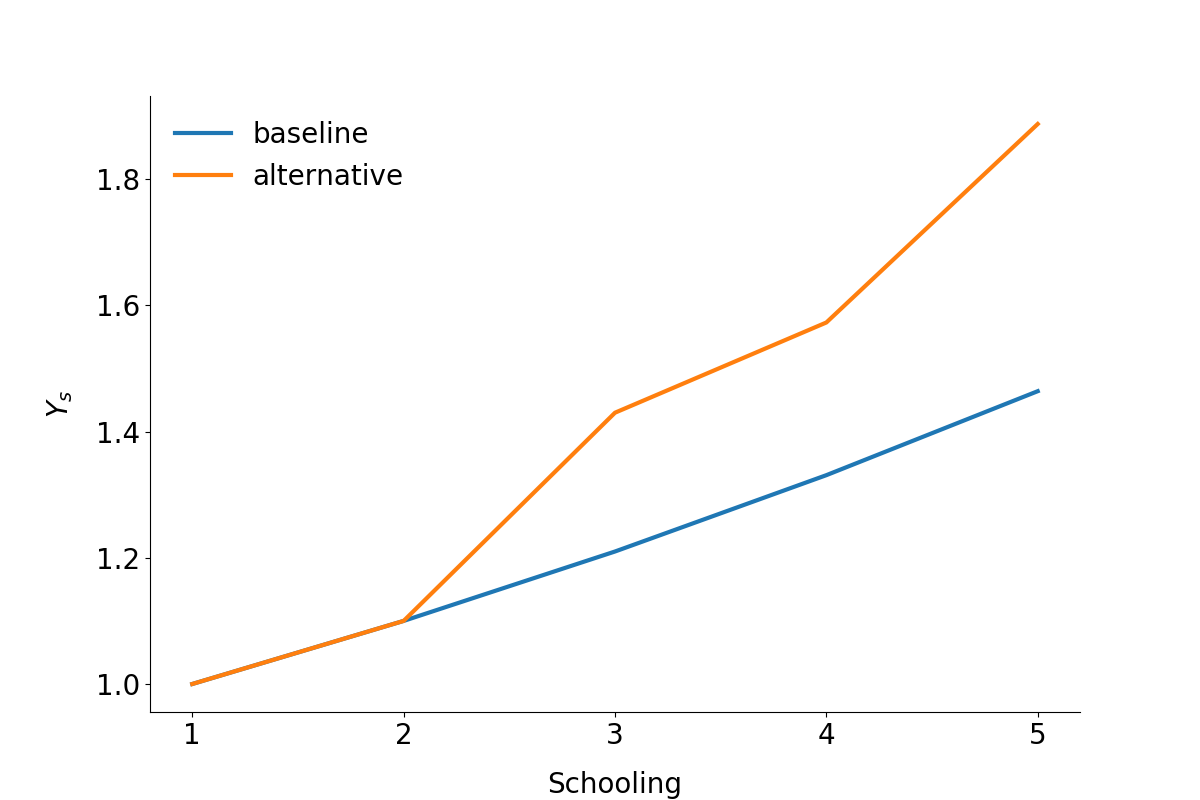
\includegraphics{fig-model-true-scenarios}}
\end{figure}
\end{frame}
%-------------------------------------------------------------------------------
%-------------------------------------------------------------------------------
\begin{frame}
We can analyze this model in a Jupyter Noteboook. Visit
\begin{center}
\url{http://bit.ly/2skwwli}
\end{center}
for the implementation.
\end{frame}
%-------------------------------------------------------------------------------
%-------------------------------------------------------------------------------
\begin{frame}
\begin{figure}[htp]\centering
\caption{Option values and uncertainty}
\scalebox{0.35}{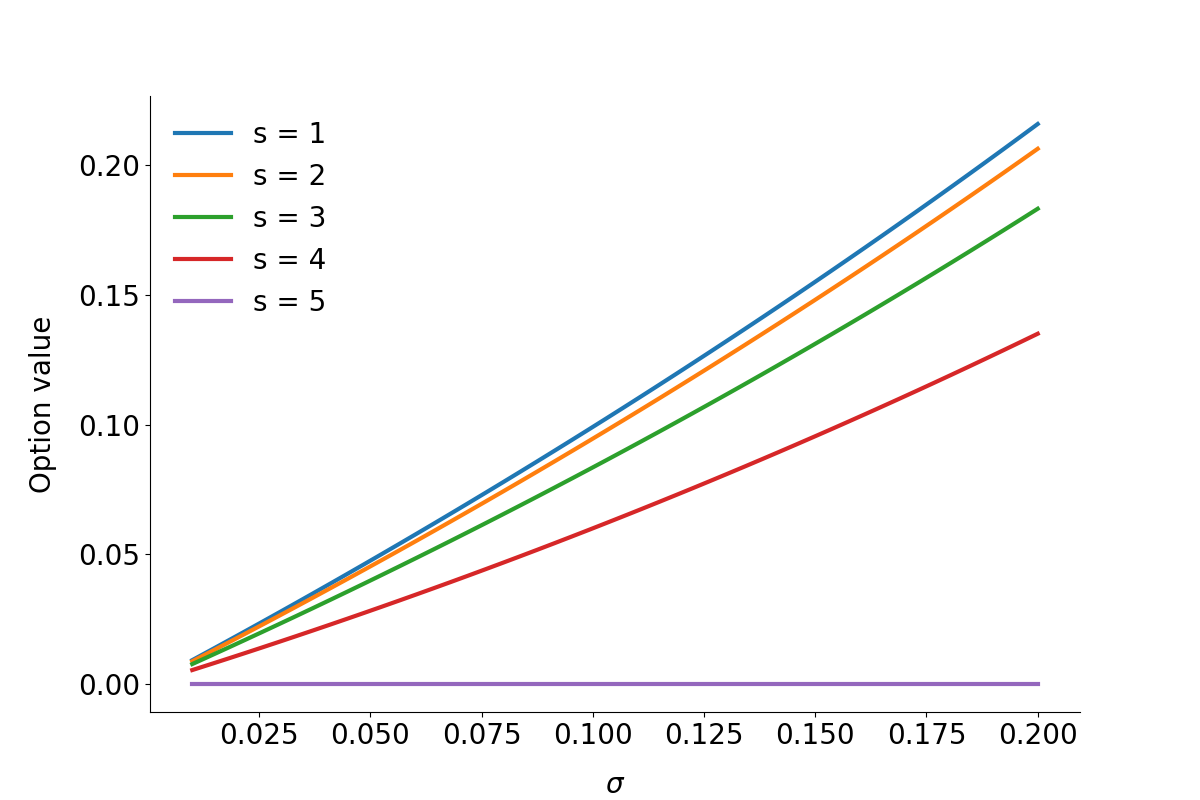
\includegraphics{fig-model-true-uncertainty}}
\end{figure}
\end{frame}
%-------------------------------------------------------------------------------
%-------------------------------------------------------------------------------
\begin{frame}
\begin{figure}[htp]\centering
\caption{Option values and sheepskin effects}
\scalebox{0.35}{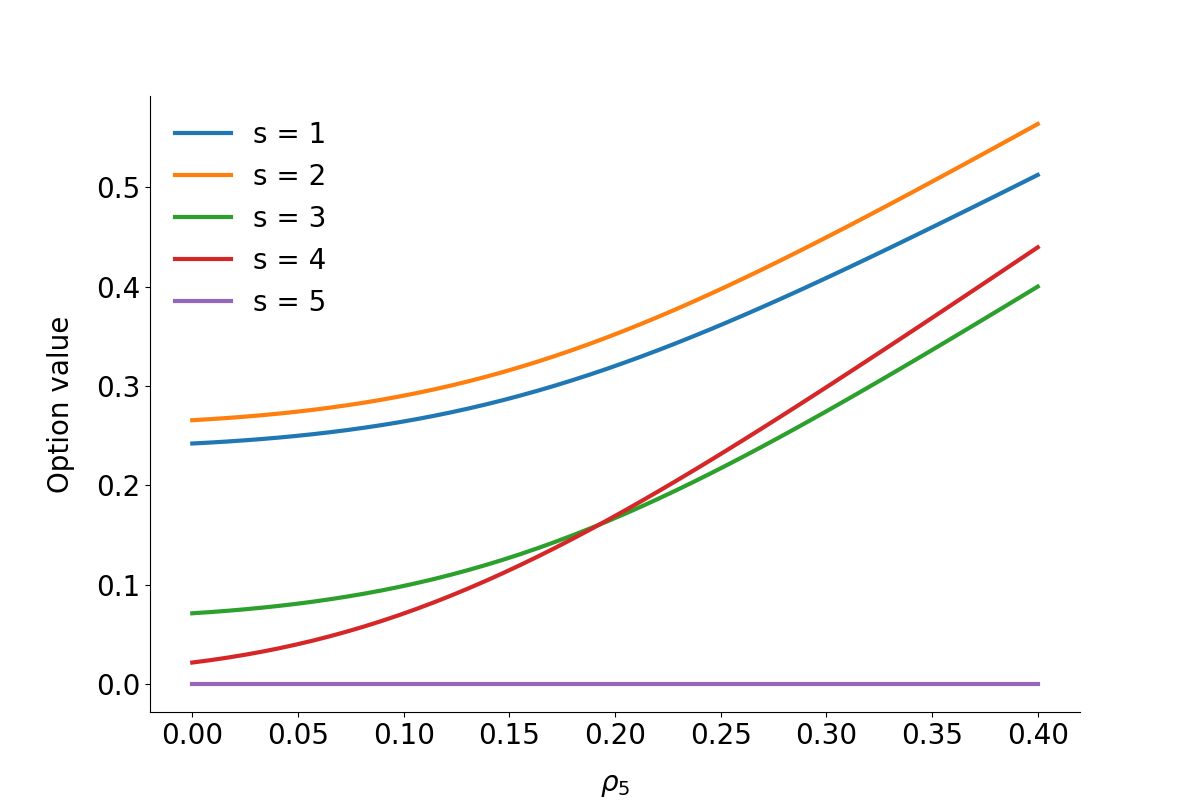
\includegraphics{fig-model-true-nonlinearities}}
\end{figure}
\end{frame}
%-------------------------------------------------------------------------------
%-------------------------------------------------------------------------------
\begin{frame}\textbf{Key features}\vspace{0.3cm}

\begin{itemize}
\item The convergence of $O_{5, 4}$ and $O_{4, 3}$ follows from the additional benefits of obtaining 5 years of schooling as we increase the growth rate $\rho_5$. It simply dominates the increase going from three to four years of schooling parameterized by $\rho_4$.
\end{itemize}

\end{frame}
%-------------------------------------------------------------------------------
%-------------------------------------------------------------------------------
\begin{frame}
\begin{figure}[htp]\centering
\caption{Returns}
\scalebox{0.35}{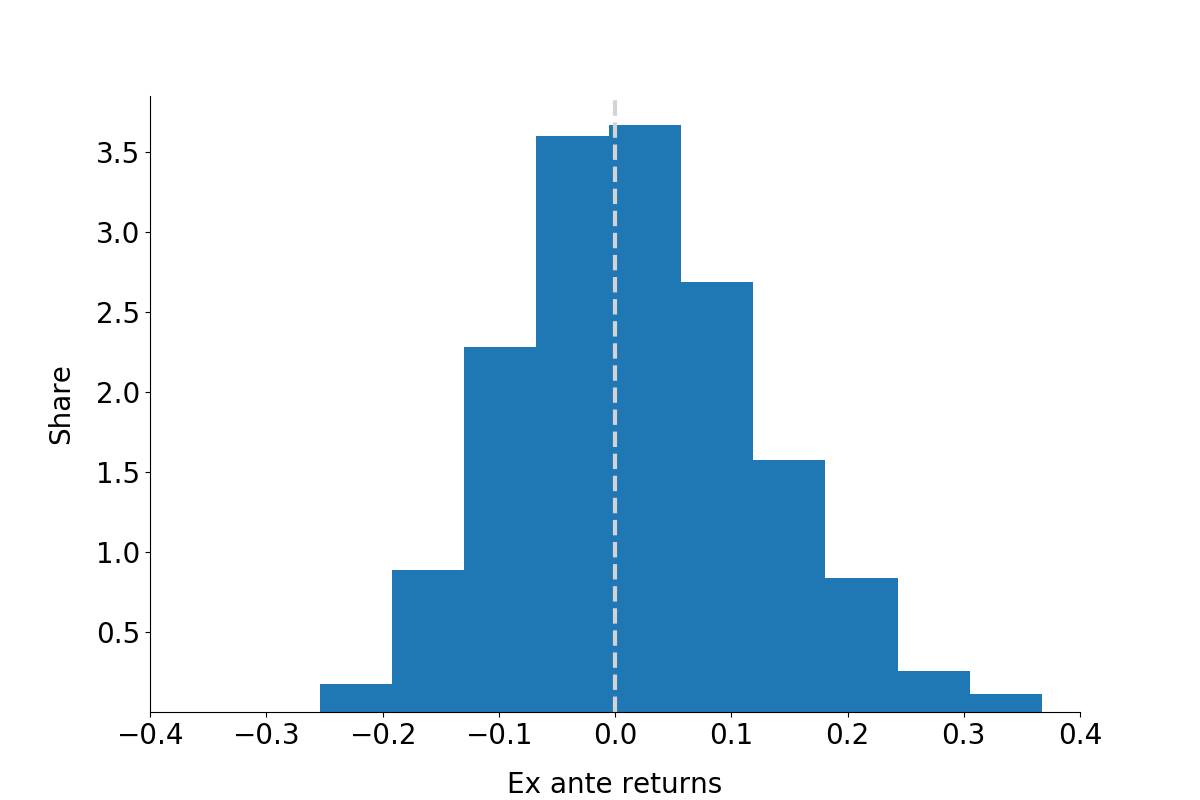
\includegraphics{fig-model-true-returns}}
\end{figure}
\end{frame}
%-------------------------------------------------------------------------------
%-------------------------------------------------------------------------------
